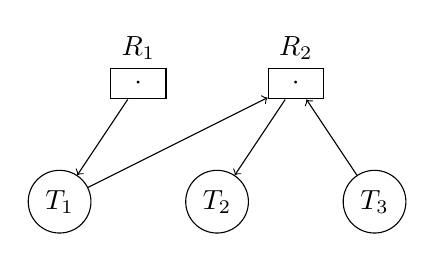
\begin{tikzpicture}
\tikzstyle{label} = [above,yshift=5pt];
\tikzstyle{res}=[minimum width=20pt,minimum height=5pt,draw];
\tikzstyle{pro}=[circle,draw];
\tikzstyle{alloc}=[->];
\node (v1) [res] at (-1,1) {$\cdot$};
\node [label] at (v1) {$R_1$};
\node [pro] (v2) at (-2,-0.5) {$T_1$};
\draw [alloc] (v1) edge (v2);

\node [pro] (v4) at (0,-0.5) {$T_2$};
\node [pro] (v5) at (2,-0.5) {$T_3$};
\node (v3) [res] at (1,1) {$\cdot$};
\node [label] at (v3) {$R_2$};
\draw [alloc] (v2) edge (v3);
\draw [alloc] (v3) edge (v4);
\draw [alloc] (v5) edge (v3);
\end{tikzpicture}